\section{Dual-Generator Adversarial Support Constraint Offline RL}

We now present our algorithm, which uses a novel dual-generator GAN in combination with a weighting method to enable GAN-based offline RL that constrains the learned policy to remain within the support of the data distribution. We call our method \textit{Dual-generator Adversarial Support Constraint Offline RL (\name{})}. We will first introduce the dual-generator training method generically, for arbitrary generators that must optimize a user-specified function $f(x)$ within the support of the data distribution in Section~\ref{sec:dual_gen}. We will then show this method can be incorporated into a complete offline RL algorithm in Section~\ref{sec:update_rule} in combination with our proposed weighting scheme, and then summarize the full resulting actor-critic method in Section~\ref{sec:algo_summary}.
%Our approach comprises four different networks: value function, policy, auxiliary generator, and discriminator. We first illustrate the benefits of dual generators in \autoref{sec:dual_gen}. \autoref{sec:update_rule} discusses the update rules for each network. In this subsection, we also motivate using the probability computed by the discriminator to weight the contribution of the value estimates in the policy objective function. Finally, we provide a step-by-step explanation of our method in \autoref{sec:algo_summary}, demonstrating GAN training can be incorporate into a standard actor-critic offline RL framework.

% https://colab.research.google.com/drive/1vD57Cbwt2xE_u8xqq0qJuOdFo6wZgjQS#scrollTo=6ssb2LhgstkQ
\subsection{Dual generator in-support optimization}
\label{sec:dual_gen}

% \begin{figure}
% \minipage{0.5\textwidth}
% \centering
%   \includegraphics[width=0.7\linewidth]{fig/single.png}
% \endminipage\hfill
% \minipage{0.5\textwidth}
% \centering
%   \includegraphics[width=0.7\linewidth]{fig/dual.png}
% \endminipage\hfill
%   \caption{Visualizations to illustrate the benefit of \textit{dual} generators over single generator when maximizing a secondary objective $f(x)$ in the GAN framework. In both figures, $p_\mathcal{D}(x)$ is the data distribution. The x-axis is an one-dimensional sample space. {\bf Left:} In this figure, since there is only a single generator, the generator $G$ is trained to jointly maximize the objective $f(x)$ and matches the data distribution $p_\mathcal{D}(x)$. The distribution $p_G$ induced by the generator is thus not very good at either maximizing the objective $f(x)$ or matching the data distribution. {\bf Right:} In this figure, we have two generators, inducing two distributions $p_G$ and $p_{aux}$. By introducing the auxiliary generator $G_{aux}$ into the GAN framework, the primary generator can better maximize the objective $f(x)$ while staying within the support of the data distribution $p_\mathcal{D}$. The mixed distribution also perfectly matches the data distribution, i.e. $ \dfrac{p_G(x) + p_{aux}(x)}{2} = p_{\mathcal{D}} (x) $. Note that in these two figures, the primary generator aims to maximize $f(x)$ (instead of minimize) to allow for more intuitive interpretation of the figures. }
%   \label{fig:dual_gen_viz}
% \end{figure}

\begin{wrapfigure}{R}{0.5\textwidth}
%  \vspace{-4em}
  \begin{center}
    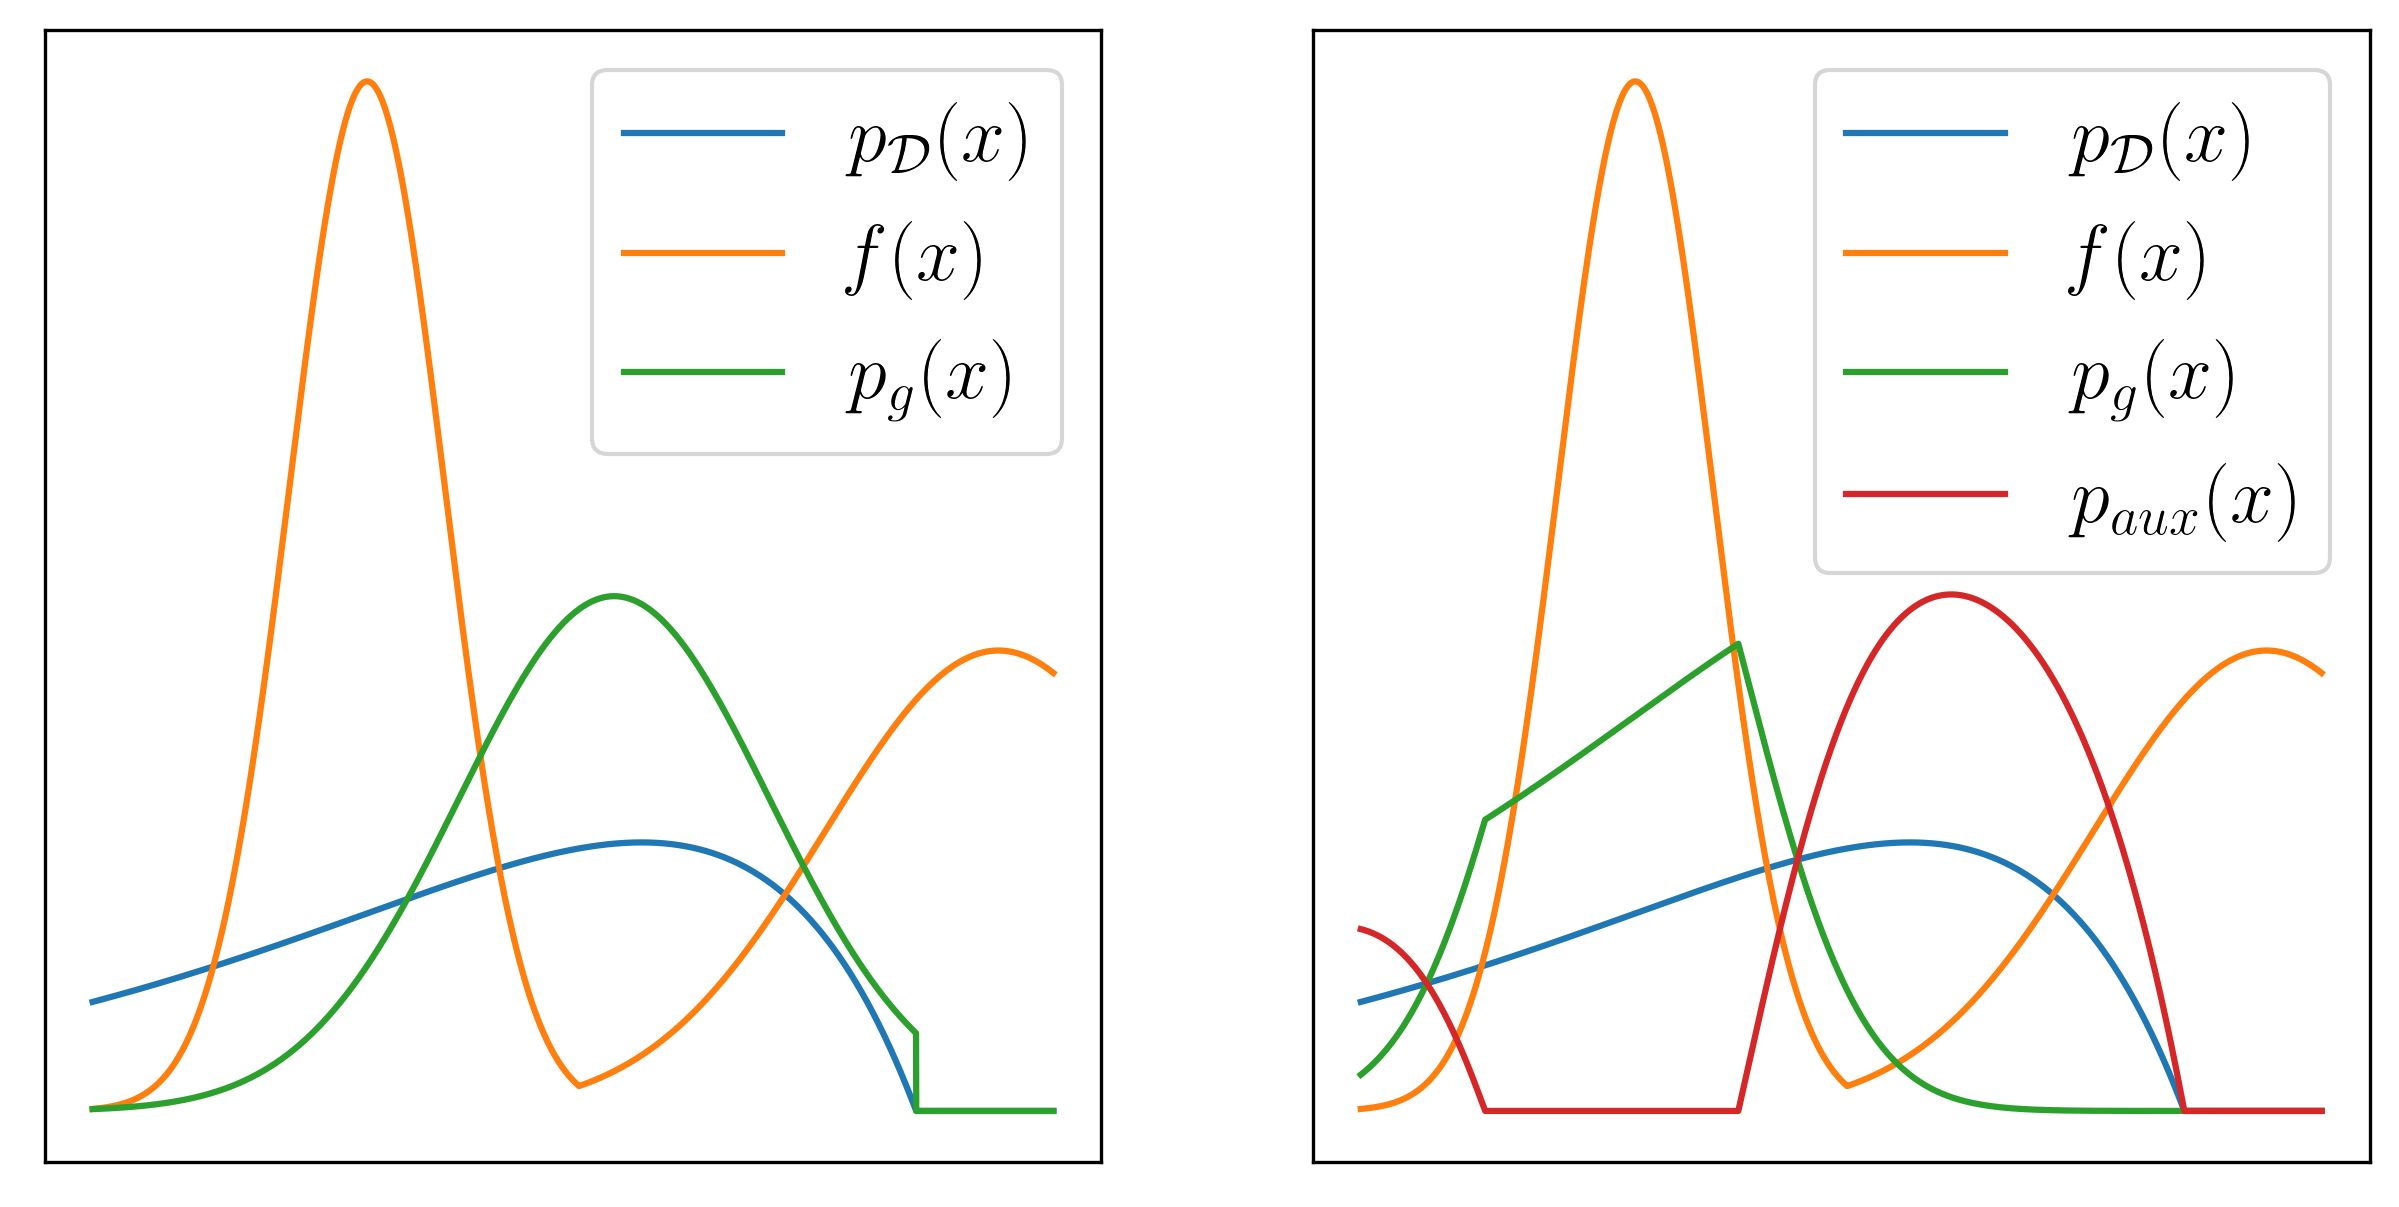
\includegraphics[width=\linewidth]{chapter_3/fig/single_and_dual.png}
  \end{center}
  \caption{Visualizations to illustrate the benefit of \textit{dual} generators over single generator when maximizing a secondary objective $f(x)$ in the GAN framework. In both figures, $p_\mathcal{D}(x)$ is the data distribution. The x-axis is a one-dimensional sample space. {\bf Left:} In this figure, since there is only a single generator, the generator $G$ is trained to jointly maximize the objective $f(x)$ and matches the data distribution $p_\mathcal{D}(x)$. The distribution $p_G$ induced by the generator is thus not very good at either maximizing the objective $f(x)$ or matching the data distribution. {\bf Right:} In this figure, we have two generators, inducing two distributions $p_G$ and $p_{aux}$. By introducing the auxiliary generator $G_{aux}$ into the GAN framework, the primary generator can better maximize the objective $f(x)$ while staying within the support of the data distribution $p_\mathcal{D}$. The mixed distribution also perfectly matches the data distribution, i.e. $ \dfrac{p_g(x) + p_{aux}(x)}{2} = p_{\mathcal{D}} (x) $. Note that in these two figures, the primary generator aims to maximize $f(x)$ (instead of minimize) to allow for more intuitive interpretation. }
  \label{fig:dual_gen_viz}
%   \vspace{-6em}
\end{wrapfigure}

% \subsection{Ensure the discriminator does not have an advantage}
In this section, we will develop an approach for performing a joint optimization of adversarial and secondary objectives of the generator in a GAN framework, which we will then apply to offline RL. This is a necessary component for performing the joint optimization in Eq.~\ref{eq:brac} without introducing a conflict of these objectives. All proofs for theorems presented in this section are in Appendix A.

Let's consider a general objective that requires training a generator $G$ to fool the discriminator $D$ while also optimizing the expected value of some other function $f$:
% \begin{align}
%     \min_{G} \max_{D}  \mathbb{E}_{ x \sim p_{\mathcal{D}}} [\log(D(x))] + \mathbb{E}_{z \sim p(z)} [\log(1-D(G(z)))]  + \mathbb{E}_{z \sim p(z)} [ f ( G(z) ) ] \label{eq:joint_nodual}
% \end{align}
\begin{align}
   \min_{G} \max_{D} \quad & \mathbb{E}_{ x \sim p_{\mathcal{D}}} [\log(D(x))] \nonumber \\
+ \hspace{0.3em} & \mathbb{E}_{z \sim p(z)} [\log(1-D(G(z)))] \nonumber \\
+ \hspace{0.3em} & \mathbb{E}_{z \sim p(z)} [ f ( G(z) ) ] \label{eq:joint_nodual}
\end{align}
where the first two terms are the same as the objective of the GAN formulation. We have also added an additional term $\mathbb{E}_{z \sim p(z)} [ f ( G(z) ) ]$, where $f$ is a mapping from the generator output to a scalar value. The third term represents a secondary objective that the generator should optimize.
\begin{restatable}{thm}{thmdisjoint}
\label{thm_disjoint}
The optimal generator of Eq.~\ref{eq:joint_nodual} induces a distribution $ p^*_g(x) = p_{\mathcal{D}} (x) \dfrac{ e^{- f(x) - \nu} }{ 2 - e^{ - f(x) - \nu } }$, where $\nu > 0$ is the Lagrange multiplier that ensures that $p^*_g(x)$ is normalized to 1.
\end{restatable}
%%SL.5.18: say where the proof for this is

We can see that by adding a secondary objective function for the generator, in general, the optimal generator does not attempt to match the data distribution $ p_{\mathcal{D}} (x) $ anymore, but instead tries to match the data distribution weighted by $ \dfrac{ e^{- f(x) - \nu } }{ 2 - e^{ - f(x) - \nu } } $. We expect that in such case, the discriminator clearly has an advantage in the two player zero-sum game and will be able to distinguish between real samples and sample generated by the generator.

To allow the generator to specialize in optimizing the secondary objective function, we propose to introduce a second auxiliary generator that matches the portion of the data distribution that is not well captured by the primary generator. Let $p_{mix} = \dfrac{ p_g + p_{aux} }{ 2 }$, consider the min-max problem:
% \begin{align}
%     \min_{G, \textcolor{red}{G_{aux}}  } \max_{D}  \mathbb{E}_{ x \sim p_{\mathcal{D}} } [\log(D(x))] + \mathbb{E}_{ \textcolor{red}{ x \sim \dfrac{ p_G + p_{aux} }{ 2 } } } [ \log(1-D(x))]  + \dfrac{1}{2} \mathbb{E}_{ x \sim p_g } [ f ( x ) ] \label{eq:joint_gan}
% \end{align}
\begin{align}
    \min_{G, G_{aux} } \max_{D}  \mathbb{E}_{ x \sim p_{\mathcal{D}} } [\log(D(x))] + \mathbb{E}_{ x \sim p_{mix} } [ \log(1-D(x))]  + \mathbb{E}_{ x \sim p_g } [ f ( x ) ], \label{eq:joint_gan}
\end{align}
%%SL.5.18: the "x \sim \dfrac{ p_G + p_{aux} }{ 2 }" looks really awkward in this Eq. -- maybe we can just define a symbol for this and use that symbol?
where we mix samples from the primary generator $G$ and the auxiliary generator $G_{aux}$ to generate samples that can fool the discriminator. The mixing is indicated by the distribution $p_{mix}$ in the second term of Eq.~\ref{eq:joint_gan}. The first and third term of Eq.~\ref{eq:joint_gan} are the same as the objective in Eq.~\ref{eq:joint_nodual}.

We next theoretically demonstrate the benefit of adding the auxiliary generator to the GAN formulation with the following Theorem.

% \begin{theorem}[Informal]
% \label{thm_joint_in_support_max}
% % Given that $f$ is appropriately bounded in its $\infty$-norm, $||f||_\infty \leq C_0 < \infty$, the primary generator $p_G$ performs in-support optimization of $f(x)$.
% % Given that $f$ is appropriately normalized, the primary generator $p_G$ performs in-support optimization of $f(x)$.
% The primary generator $p_G$ performs in-support optimization of $f(x)$.
% \end{theorem}
\begin{restatable}[Informal]{thm}{thmjointinsupportmax}
\label{thm_joint_in_support_max}
% Given that $f$ is appropriately bounded in its $\infty$-norm, $||f||_\infty \leq C_0 < \infty$, the primary generator $p_G$ performs in-support optimization of $f(x)$.
% Given that $f$ is appropriately normalized, the primary generator $p_G$ performs in-support optimization of $f(x)$.
The primary generator $p_G$ performs in-support optimization of $f(x)$.
\end{restatable}


We first note that the optimal solution of the mixed distribution from Eq.~\ref{eq:joint_gan} is the real data distribution:
\begin{align}
\dfrac{ p^*_{aux} (x) + p^*_{g} (x) }{2} = p_{\mathcal{D} } (x)
\label{eq:joint_match_real}
\end{align}
Accordingly, the optimal auxiliary generator distribution can be expressed as 
%%SL.5.18: if you find you are out of space, you can easily make some of these Eq.s inline
\begin{align}
    p^*_{aux} (x) = 2 p_{\mathcal{D}} (x) - p^*_g(x) \label{eq:paux_dist}
\end{align}
Let $x_0$ to be the element inside the support of the data distribution $p_{\mathcal{D}}$ that minimizes $f$. That is: $$ x_0 = \underset{x \in \text{Supp}( p_{\mathcal{D}} ) }{\arg\min} f(x) $$
When optimizing the secondary objective $f(x)$, the primary generator will maximize the probability mass of in-support samples that maximize $f(x)$. However, Eq.~\ref{eq:paux_dist} introduces a constraint that enforces $ 2 p_{\mathcal{D}} (x) - p^*_g(x) \geq 0$ for $p^*_{aux} (x) \geq 0$ to remain a valid distribution. This leads us to conclude that the optimal primary generator $p^*_g$ assigns the following probability to $x_0$:
% This leads us to the following definition of the in-support global maximum $x_0$ of $f(x)$:
%%SL.5.18: Perhaps we need to rephrase the above a little -- it's not clear if this is defining what "in support global maximum" means, or if it's stating a theorem saying what p*_g will learn. In fact, it's actually kind of doing both, which is really awkward -- it's simultaneously a definition for in-support max (left side) and stating a result without proof (right side). Maybe split this into a definition for in-support and a theorem statement (the right side) with proof in the appendix?
\begin{align}
    p^*_{g} (x_0) & = \begin{cases}
    2p_{\mathcal{D}} (x_0) \quad  \text{if} \quad 2p_{\mathcal{D}} (x_0) < 1 \\
    1 \quad \quad  \quad \quad \text{otherwise}
    \end{cases}
\end{align}
Interestingly, if the global maximum $x_0$ is not taking the full probability mass, the rest of the probability mass is redistributed to the next best in-support maxima, which we can define recursively:
\begin{align}
         \text{For} \,\, x_i \in \underset{x \in \text{Supp}( p_{\mathcal{D}} )  \setminus \{ x_j \}_{j=0}^{i-1} }{\arg\min} f(x), \,\,
    p^*_{g} (x_i) & = \begin{cases}
      2p_{\mathcal{D}} (x_i)\quad \quad \quad \quad \quad \text{if} \quad \sum_{j=0}^i p^*_g(x_j) < 1 \\
      1 -  \sum_{j=0}^{i-1} p^*_g(x_j) \quad \,\, \text{if} \quad \sum_{j=0}^i p^*_g(x_j) > 1 \\ 
      0 \quad \quad \quad \quad \quad \quad \quad \quad  \text{if} \quad \sum_{j=0}^{i-1} p^*_g(x_j) = 1 
    \end{cases}
    \label{eq:sol_3_cases}
\end{align}

We provide more explanation for the solution in Eq.~\ref{eq:sol_3_cases}. 
In the first case, $p^*_{g} (x_i) = 2p_{\mathcal{D}} (x_i)$ if $\sum_{j=0}^i p^*_g(x_j) < 1$. 
That is, if the optimal solution for the primary generator $p^*_{g}$ \textit{can} assign the probability $2p_{\mathcal{D}} (x_i)$ to the $i^{th}$ in support minima of $f(x)$ without the total sum of probability assigned $\sum_{j=0}^i p^*_g(x_j)$ going over $1$, then the primary generator $p^*_{g}$ will assign the probability $2p_{\mathcal{D}} (x_i)$ to $x_i$. 

In the second case, $p^*_{g} (x_i) = 1 -  \sum_{j=0}^{i-1} p^*_g(x_j)$ if $\sum_{j=0}^i p^*_g(x_j) > 1$. That is, if by assigning the probability $2p_{\mathcal{D}} (x_i)$ to the $i^{th}$ in support minima of $f(x)$, the total sum of probability assigned $\sum_{j=0}^i p^*_g(x_j)$ \textit{goes over} $1$, then the primary generator $p^*_{g}$ will assign the remaining probability $1 -  \sum_{j=0}^{i-1} p^*_g(x_j)$ to $x_i$. In the third case, the generator assigns probability $0$ to $x_i$ because all the probability has already been assigned. 
% \begin{theorem}
% The optimal solutions for the primary and secondary generators are:
% \begin{align}
%     p^*_{aux} (x) & = 2 p_{\mathcal{D}} (x) - p^*_g(x) \\
%     \text{For} \quad x_0 \in \underset{x \in Supp( p_{\mathcal{D}} ) }{argmax} f(x), \quad 
%     p^*_{g} (x_0) & = \begin{cases}
%     2p_{\mathcal{D}} (x_0) \quad  \text{if} \quad 2p_{\mathcal{D}} (x_0) < 1 \\
%     1 \quad \text{otherwise}
%     \end{cases} \\ 
%      \text{We then define $p^*_{g}$ recursively, for }  x_i \in \underset{x \in Supp( p_{\mathcal{D}} )  \setminus \{ x_j \}_{j=0}^{i-1} }{argmax} f(x): \\
%     p^*_{g} (x_i) & = \begin{cases}
%       2p_{\mathcal{D}} (x_i) \quad \text{if} \quad \sum_{j=0}^i p^*_g(x_j) < 1 \\
%       1 -  \sum_{j=0}^{i-1} p^*_g(x_j) \quad \text{if} \quad \sum_{j=0}^i p^*_g(x_j) > 1 \\ 
%       0 \quad \quad \text{if} \quad \sum_{j=0}^{i-1} p^*_g(x_j) = 1 
%     \end{cases}       
% \end{align}
% \end{theorem}
%     % p^*_{g} (x) & = \dfrac{1}{Z_{G}} \left[ 2 p_{\mathcal{D} } (x) \dfrac{ e^{2f(x)} }{ 2 - e^{ 2f(x) } } - p^*_{aux} (x) \right] 

% \textcolor{red}{Does anyone have a nicer way to write the expression above}.

% \textcolor{red}{TODO: show that the dual generator optimal solution is indeed preferable to single generator, maybe in terms of well the primary generator can maximize E[f(x)]}. We probably need to introduce a mixing weight $\alpha$ between the two generators show this.

% TODO: provide some intuition about why the solution for $p^*_g$ looks like that, this is because $p^*_{aux} (x) = 2 p_{\mathcal{D}} (x) - p^*_g(x) \geq 0$, so $p^*_g(x)$ can be at most $2p_{\mathcal{D}} (x)$. And $p_{\mathcal{D}} (x) = 0 \implies p^*_{aux} (x) = p^*_g(x) = 0 $. As such, let $x_0$ be the global maxima of $f(x)$ that lies within the support of $p_{\mathcal{D}}$, we set the probability of the global maxima to be $2p_{\mathcal{D}}(x_0)$. If this value is less than 1, that means we still have probability mass left to redistribute. We then consider the next global maxima $x_1$ of $f(x)$ that lies within the support of $p_{\mathcal{D}}$, excluding $x_0$, and set the probability of the $p^*_{g} (x_1)$ to be $2p_{\mathcal{D}}(x_0)$. So on until we run out of probability mass to redistribute.

% \begin{corollary}
% $ \dfrac{ p^*_{aux} (x) + p^*_{g} (x) }{2} = p_{\mathcal{D} } (x) $
% \end{corollary} 


To summarize the benefit of dual generator, we note that by introducing an auxiliary generator and mixing it with the primary generator, not only does the optimal solution for the mixed distribution match the real data distribution, but also the primary generator can better optimize the secondary objective $f$ on the part of the domain of $f$ that is within the support of the data distribution $p_\mathcal{D}$. To better illustrate the benefit, we provide a visual explanation of the benefit in Figure~\ref{fig:dual_gen_viz}.
% in-distribution support.

% \begin{theorem}
% By allowing in-support optimization of $f(x)$, using the auxiliary generator enables the primary generator to better optimize the secondary objective $f(x)$ compared to not using the auxiliary generator and only using a single generator.
% \end{theorem}
% %%SL.5.18: we probably need a more formal statement here than just "better"
% That is, let $p_{\mathlarger{g}}^*$ be the distribution induced by the optimal generator obtained from Eq.~\ref{eq:joint_gan} where we use the auxiliary generator. Also let $p_{\mathlarger{s}}^*$ be the distribution induced by the optimal generator obtained from Eq.~\ref{eq:joint_nodual}, where we do not use the auxiliary generator. We are then interested in showing that:
% \begin{align*}
%     \mathbb{E}_{ x \sim p_{\mathlarger{g}}^* } [ f ( x ) ] \geq \mathbb{E}_{ x \sim p_{\mathlarger{s}}^* } [ f ( x ) ]
% \end{align*}
%%SL.5.18: I think the above should all be part of the theorem? that woudl make it more precise, then say where the proof is...

% We next illustrate the benefit of introducing the auxiliary generator on a toy 2D task.

% In this subsection, we show that by using a single generator, the discriminator has an advantage because the generator is not even trying to match the data distribution.

% That is, when there is a secondary objective function and we only use a single generator, then the optimal solution for the generator does not try to match the data distribution p\_data, which is what a GAN Generator should do.

% We then show that by introducing the second auxiliary generator, the mixed distribution of the first and the second generator is trying to match the data distribution, and hence the discriminator does not have an advantage anymore.

% More info: pls see file 'discriminator does not have advantage.pdf' for derivation and file 'GAN dual discriminator toy example.pdf' for the toy example

% \subsection{Support Constraint}

% In this subsection, we show a second benefit of having the second auxiliary generator. "I can show that for 2 different actions, if they have the same probability under the behavior policy, and one has higher Q value, then by having two generators, the policy can assign more mass to the higher action, as compared to when there is only one generator!"

\subsection{Update rules for offline reinforcement learning}
\label{sec:update_rule}

We will now incorporate the dual-generator method to train policies for offline RL, based on optimizing the joint objective from Eq.~\ref{eq:joint_gan}. The updates for the actor and the critic are generally similar to Eq.~\ref{eq:brac_update}. However, simply combining Eq.~\ref{eq:joint_gan} and Eq.~\ref{eq:brac_update} can still allow the policy to exploit errors in the value function during the policy improvement step. We therefore augment the policy improvement step with an adaptive weight on the Q-value.
%%SL.5.18: Maybe it would be better to have a separate subsection before this that first motivates and then explains the weighting, and then have this section just be a "putting it together" kind of algorithm summary? Or we can keep it as-is, but then it would be good to motivate the weighting somewhere before this, otherwise it's pretty surprising that we're not just plugging the Sec 4.1 thing in here but doing something more complex. Perhaps that could be done simply by taking some of the motivation that is already here and putting it earlier? Or just explicitly say that we could simply plug the GAN from 4.1 into actor-critic Eq ??, but this would have a problem, so we also do this weight (which would be most similar to the current phrasing, just a bit more explicit)
More concretely, as the policy improvement step samples actions from the current policy iterate $\policy^k$ to optimize the policy objective, there is a non-zero probability that the sampled actions will exploit spurious maxima in the value function and have their probability of being sampled again in the future increased. If the same actions are sampled during the policy evaluation step, the errors in the value functions from the next states are backed up into the preceding states, leading to divergent value functions, as we observe in our experiments. To alleviate this issue, we use the probability assigned to the sampled actions by the discriminator to weight the value function estimates in the policy objective, leading to the following updates:
\begin{align}
    Q^{k+1} \leftarrow& \argmin_{Q} \E_{s, a, s' \sim \mathcal{D}}\left[ \left((R(s, a) +  \gamma \E_{a' \sim {\policy}^k(a'|s')}[Q^{k}(s', a')]) - Q_{target}(s, a)\right)^2 \right] \label{eq:dasco_q}\\ 
    \policy^{k+1} \leftarrow& \argmax_{\policy} \E_{s, a_{\mathcal{D}} \sim \mathcal{D}, a \sim \policy^k(a|s)}\left[ \dfrac{ D^k(s,a) }{ D^k( s,a_{\mathcal{D}}(s)) }Q^{k+1}(s, a) + \log D^k(s,a) \right],
    \label{eq:dasco_pi}
\end{align}
where $ a_{\mathcal{D}}(s) $ is the action from the offline dataset. 
%The state $\bs$ is sampled from the offline dataset. The action $\ba$ is sampled from the $k^{th}$ policy iterate $ \pi^k_\phi $. 
The term $ D^k(s,a) $ down-weights the contribution of the gradient of the value function to the policy update if the discriminator deems the sampled action too unlikely. We further calibrate the probability $ D^k(s,a) $ by dividing it with the probability $ D^k(s,a_{\mathcal{D}}(s)) $ that the discriminator assigns to the dataset action $a_{\mathcal{D}}(s) $. It should be noted that during optimization the gradients are not propagated into these weights.%\autoref{eq:update_dynamic_weight} illustrate the update rule using a single state from the dataset for clarity. In practice, we average the gradient over multiple states and also incorporate a learning rate.

Next, we define the update rules for the auxiliary generator and the discriminator. We mix the samples from the $k^{th}$ iterate of the policy $\pi^k$ and the distribution $p_{aux}$ induced by the $k^{th}$ iterate of the auxiliary generator $G^k_{aux}$, that is, let $p_{mix} = \dfrac{ \pi^k + p_{aux} }{ 2 }$. At every iteration $k$, we update the $k^{th}$ iterate of the auxiliary generator $ G^{k}_{aux} $ and discriminator $D^k$ using the objectives:
\begin{align}
    G^{k+1}_{aux} \leftarrow& \argmin_{ G_{aux} } \mathbb{E}_{ x \sim p_{mix} } [ \log(1-D^k(s,a))] \label{eq:dasco_gaux}\\ 
    D^{k+1}  \leftarrow& \argmax_{D}  \mathbb{E}_{ x \sim p_{\mathcal{D}} } [\log(D^k(s,a))] + \mathbb{E}_{ x \sim p_{mix} } [ \log(1-D^k(s,a))]\label{eq:dasco_d}
    %%SL.5.18: same comment about the akwardness of the giant mixture Eq. in the subscript
\end{align}
%%SL.5.18: perhaps pseudocode summarizing the whole algorithm would be useful? maybe together with a short paragraph after this that just rounds out all the pieces and summarize the whole thing
\subsection{Algorithm summary}
\label{sec:algo_summary}

Algorithm ~\ref{algo:dasco} provides a step-by-step description of our algorithm. At every training step, we sample a batch of transitions from the offline dataset and proceed to update the parameters of the value function, the policy, the auxiliary generator and the discriminator in that order.

\begin{algorithm}[H]
\begin{algorithmic}[1]
\State{Initialize Q-function $Q_\theta$, policy $\pi_\phi$, auxiliary generator $G_{aux, \psi}$, discriminator $D_\omega$}
\For{training step $k$ in \{1,\dots,N\}}
\State{$(s, a, r, s') \gets \mathcal{D}$: Sample a batch of transitions from the dataset}
\State{$\theta^{k+1} \gets$ Update Q-function $Q_\theta$ using the Bellman update in Eq.~\ref{eq:dasco_q}}
\State{$\phi^{k+1} \gets$ Update policy $\pi_\phi$ using the augmented objective in Eq.~\ref{eq:dasco_pi}}
\State{$\psi^{k+1} \gets$ Update auxiliary generator $G_{aux, \psi}$ using the objective in Eq.~\ref{eq:dasco_gaux}}
\State{$\omega^{k+1} \gets$ Update discriminator $D_\omega$ using mixed samples from $\pi_\phi$ and $G_{aux, \psi}$ as in Eq.~\ref{eq:dasco_d}}
\EndFor
\caption{\name{} algorithm summary}
\label{algo:dasco}
\end{algorithmic}
\end{algorithm}